% $Header: /cvsroot/latex-beamer/latex-beamer/solutions/generic-talks/generic-ornate-15min-45min.en.tex,v 1.5 2007/01/28 20:48:23 tantau Exp $

\documentclass{beamer}

\usepackage{caption}
\captionsetup{labelformat=empty,labelsep=none,font=scriptsize}
\setlength{\abovecaptionskip}{0pt}

\usepackage{color}
%% These definitions are based on darkred at
%% http://www.december.com/html/spec/colorcmyk.html
\definecolor{darkred}{cmyk}{0, 1, 1, 0.45}
\newcommand{\jul}{\textcolor{darkred}}
\newcommand{\jan}{\textcolor{blue}}

% This file is a solution template for:

% - Giving a talk on some subject.
% - The talk is between 15min and 45min long.
% - Style is ornate.



% Copyright 2004 by Till Tantau <tantau@users.sourceforge.net>.
%
% In principle, this file can be redistributed and/or modified under
% the terms of the GNU Public License, version 2.
%
% However, this file is supposed to be a template to be modified
% for your own needs. For this reason, if you use this file as a
% template and not specifically distribute it as part of a another
% package/program, I grant the extra permission to freely copy and
% modify this file as you see fit and even to delete this copyright
% notice. 


\mode<presentation>
{
  \usetheme{Warsaw}
  % or ...

  \setbeamercovered{transparent}
  % or whatever (possibly just delete it)
}


\usepackage[english]{babel}
% or whatever

\usepackage[latin1]{inputenc}
% or whatever

\usepackage{times}
\usepackage[T1]{fontenc}
% Or whatever. Note that the encoding and the font should match. If T1
% does not look nice, try deleting the line with the fontenc.


%% \title[Short Paper Title] % (optional, use only with long paper titles)
%% {Presentation Title}
%% \title[]{Initial findings}
%\subtitle {Eastern CASTNET sites, May-Sep.~2001} % (optional)

%% \author[Author, Another] % (optional, use only with lots of authors)
%% {F.~Author\inst{1} \and S.~Another\inst{2}}
%% % - Use the \inst{?} command only if the authors have different
%% %   affiliation.
%% \author[Swall et al.]{Jenise Swall\inst{1}, Ana Rappold\inst{2}, and Lucas Neas\inst{2}
% - Use the \inst{?} command only if the authors have different
%   affiliation.

%% \institute[Universities of Somewhere and Elsewhere] % (optional, but mostly needed)
%% {
%%   \inst{1}%
%%   Department of Computer Science\\
%%   University of Somewhere
%%   \and
%%   \inst{2}%
%%   Department of Theoretical Philosophy\\
%%   University of Elsewhere}
%% % - Use the \inst command only if there are several affiliations.
%% % - Keep it simple, no one is interested in your street address.
 %% \institute[VCU]
 %% {
 %%   \inst{1}%
 %%   Dept.\ of Statistical Sciences and Operations Research\\
 %%   Virginia Commonwealth University
 %%   \and
 %%   \inst{2}%
 %%   National Health and Environmental Effects Research Laboratory\\
 %%   U.S.~Environmental Protection Agency
 %% }

%% \date[Short Occasion] % (optional)
%% {Date / Occasion}
%% \date{Oct.\ 2017}

%% \subject{Talks}
% This is only inserted into the PDF information catalog. Can be left
% out. 



% If you have a file called "university-logo-filename.xxx", where xxx
% is a graphic format that can be processed by latex or pdflatex,
% resp., then you can add a logo as follows:

% \pgfdeclareimage[height=0.5cm]{university-logo}{university-logo-filename}
% \logo{\pgfuseimage{university-logo}}



% Delete this, if you do not want the table of contents to pop up at
% the beginning of each subsection:
\AtBeginSection[]
{
  \begin{frame}<beamer>{Outline}
    \tableofcontents[currentsection,currentsubsection]
  \end{frame}
}


% If you wish to uncover everything in a step-wise fashion, uncomment
% the following command: 

%\beamerdefaultoverlayspecification{<+->}

\useoutertheme{infolines}

\begin{document}

%% \begin{frame}
%%   \titlepage
%% \end{frame}

\begin{frame}{Outline}
  \tableofcontents
  % You might wish to add the option [pausesections]
\end{frame}


% Since this a solution template for a generic talk, very little can
% be said about how it should be structured. However, the talk length
% of between 15min and 45min and the theme suggest that you stick to
% the following rules:  

% - Exactly two or three sections (other than the summary).
% - At *most* three subsections per section.
% - Talk about 30s to 2min per frame. So there should be between about
%   15 and 30 frames, all told.


%% %%%%%%%%%%%%%%%%%%%%%%%%%%%%%%%%%%%%%%%%%%%%%%%%%%%%%%%%%%



%% %%%%%%%%%%%%%%%%%%%%%%%%%%%%%
%% Introductory material
%% \section[Background]{Background ideas and info}
\section[Preparation]{Preparing the data}


\begin{frame}{Initial looks into family taxa}

  \noindent Data was read from Excel files:\\
  \texttt{HenleyLake\_Taxonomy.xlsx} - taxonomy info\\
  \texttt{HenleyLake\_SampleInformation.xlsx} - sample info (degdays, type, date)

  \vspace{0.1in}

  \noindent Family data from \texttt{Taxlevel 5-Family} worksheet
  \begin{itemize}
  \item Ribs: 154 family-level taxa represented
  \item Scapulae: 210 family-level taxa represented
  \item Water: 216 family-level taxa represented
  \end{itemize}
 
\end{frame}



\begin{frame}{Percentages unclassifed at the family level}

  \begin{center}
    \begin{figure}
      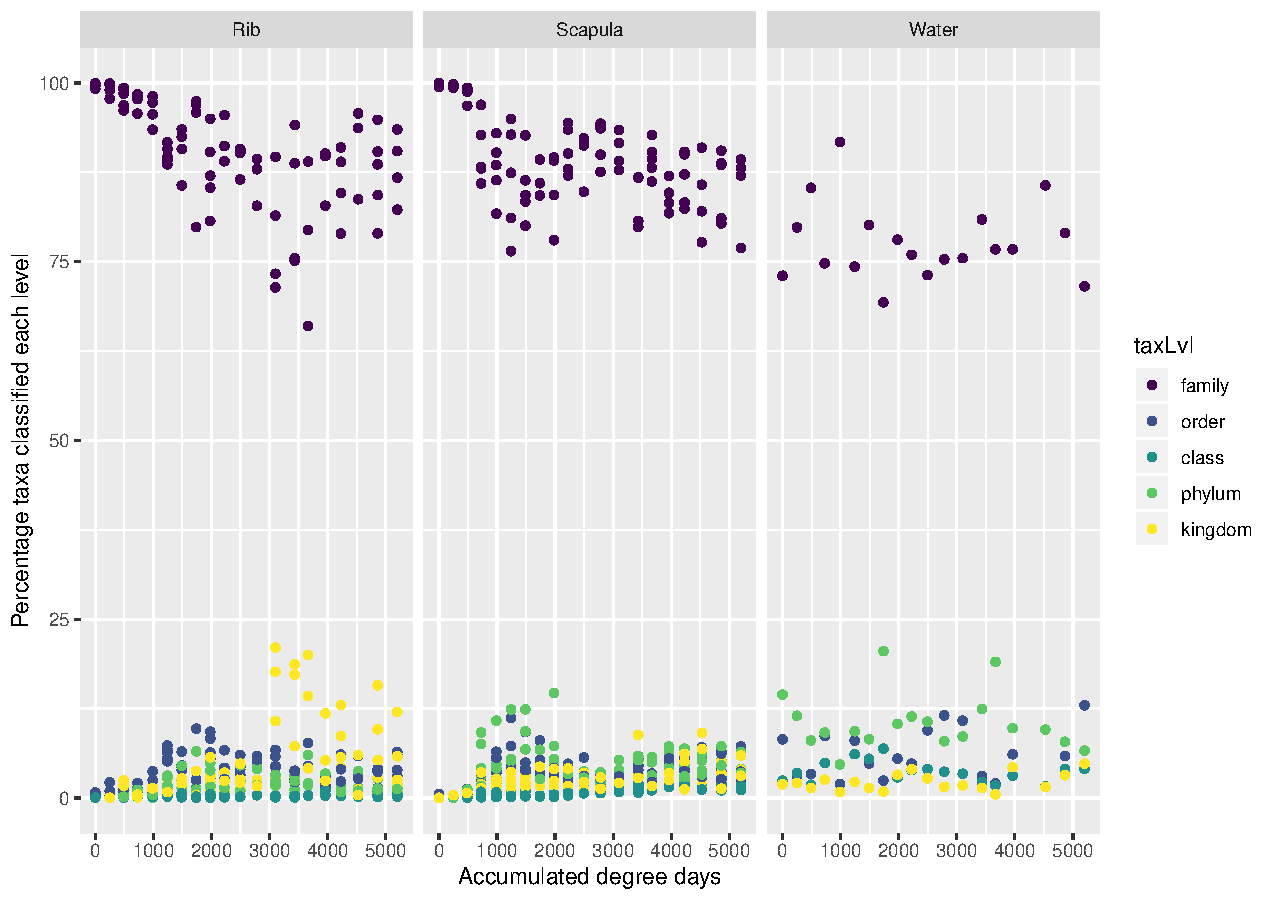
\includegraphics[width=3.25in]{family_perc_classif_by_add_type}
    \end{figure}
  \end{center}
  \vspace{-0.1in}
  {\footnotesize
  \begin{itemize}
    \item Percentages classified to family level: 90.5\% (ribs), 88.9\%
    (scapulae), 77.7\% (water).
    \item For ADD above 3000, rib samples had a high percentage of
  counts that could only be classified at the kingdom level.
  \end{itemize}
  }
\end{frame}



\begin{frame}{Which taxa were included?}

  \noindent For each sample, we calculated the total counts of all classified,
family-level taxa.  Then, for each sample, we calculated the fraction of counts
associated with each family-level taxa.  (Raw counts were \textbf{not} used.)

  \vspace{0.1in}

  \noindent To be included in the family-level analysis, we require that a taxon
  makes up more than 1\% of the total counts for at least 2 samples.

  \vspace{0.1in}

  \noindent This is similar to the process we used when setting up for the
analyses in the Forger et al.~ paper, but we may want to revisit it.  (Should we
require more than 1\%?  For more than 2 samples?))

  \vspace{0.1in}

  \noindent Number of taxa utilized in random forest models:
  \begin{itemize}
    \item Ribs: 24 taxa
    \item Scapulae: 34 taxa
    %% \item Water: 31 taxa
  \end{itemize}


\end{frame}
%% %%%%%%%%%%%%%%%%%%%%%%%%%%%%%



%% %%%%%%%%%%%%%%%%%%%%%%%%%%%%%
\section[Ribs, family-level]{Family-level analysis for ribs}

\begin{frame}{Implementing random forest model}

\begin{itemize}
\item The model utilized 24 family-level taxa.
\item Cross-validation was used to determine that the best number of taxa to
consider at each "branching" was about 14.
\item If we were to change our critera and reduce the number of taxa which are
considered plentiful enough to be considered, then we would need to do
cross-validation again (as we might expect it to be lower than 14.)
\end{itemize}

\vspace{0.1in}

\noindent For the fitted model (using all available data):\\
\noindent RMSE: 517.0 $\pm$ 6.3  \hspace{0.05in}  Explained variation: 89.5\%
$\pm$ 0.3\%


\end{frame}



\begin{frame}{Which taxa are influential in the random forest model?}

  \begin{center}
    \begin{figure}
      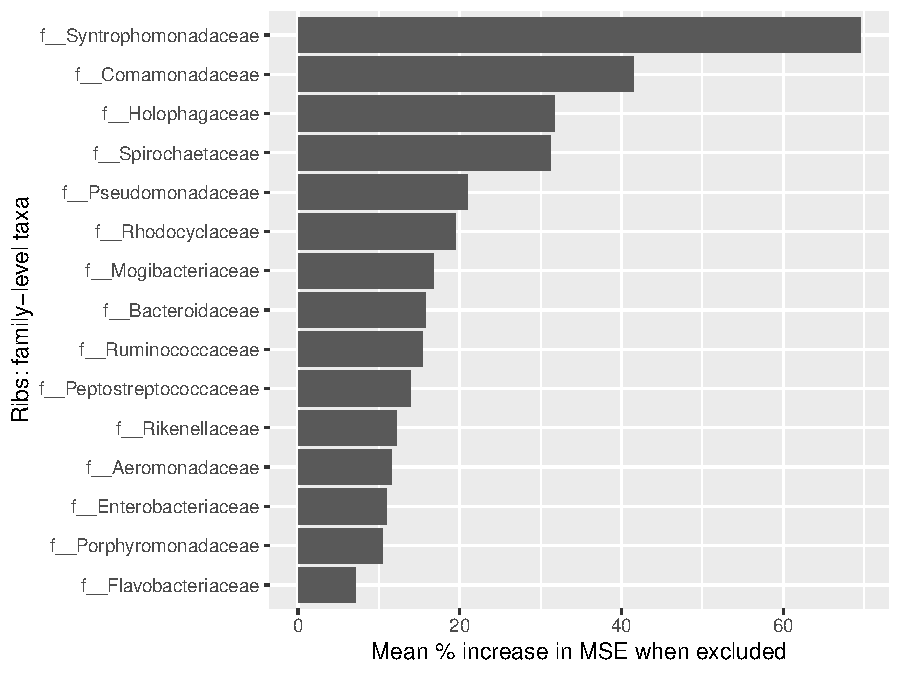
\includegraphics[width=3.25in]{use_families/w_ribs/families_rib_PercIncMSE_barchart}
    \end{figure}
  \end{center}
  \vspace{-0.1in}
  {\scriptsize
  \begin{itemize}
  \item The measure of importance is the mean percentage increase in the
    mean-square error of model predictions when the variable is left out of the
    model. 
  \item I've shown 15 because they would fit, but 24 were used in the model.
  \item The first four taxa are noticeably more influential than those that
  follow.
  \end{itemize}
  }

\end{frame}


\begin{frame}{Scatterplots for influential taxa}

  \begin{center}
    \begin{figure}
      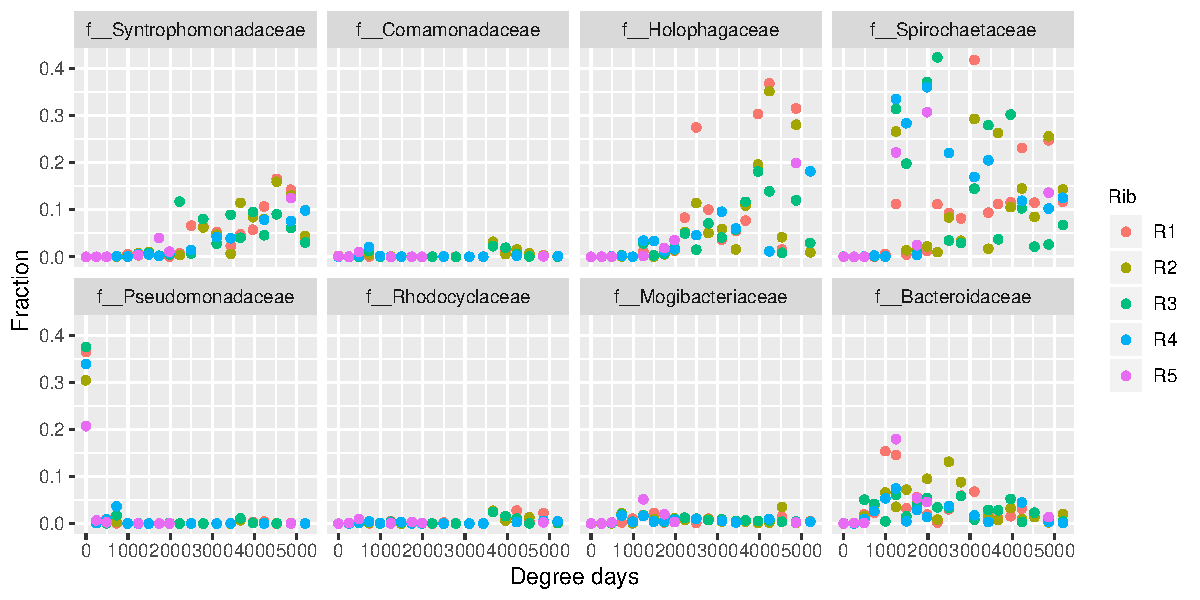
\includegraphics[width=4.75in]{use_families/w_ribs/infl_rib_family_scatter}
    \end{figure}
  \end{center}
  \vspace{-0.25in}
  {\scriptsize
  \begin{itemize}
  \item I've only shown top 6 because more than that is hard to fit.
  \item Note that the y-axes have differing scales.
  \item Fractions of Comamonadaceae and Rhodocyclaceae are very low.
  \end{itemize}
  }

\end{frame}
%% %%%%%%%%%%%%%%%%%%%%%%%%%%%%%


%% %%%%%%%%%%%%%%%%%%%%%%%%%%%%%
\section[Scapulae, family-level]{Family-level analysis for scapluae}

\begin{frame}{Implementing random forest model}

\begin{itemize}
\item The model utilized 34 family-level taxa.
\item Cross-validation was used to determine that the best number of taxa to
consider at each "branching" was about 20.
\item If we were to change our critera and reduce the number of taxa which are
considered plentiful enough to be considered, then we would need to do
cross-validation again (as we might expect it to be lower than 20.)
\end{itemize}

\vspace{0.1in}

\noindent For the fitted model (using all available data):\\
\noindent RMSE: 333.48  \hspace{0.05in}  Explained variation: 95.35\%


\end{frame}



\begin{frame}{Which taxa are influential in the random forest model?}

  \begin{center}
    \begin{figure}
      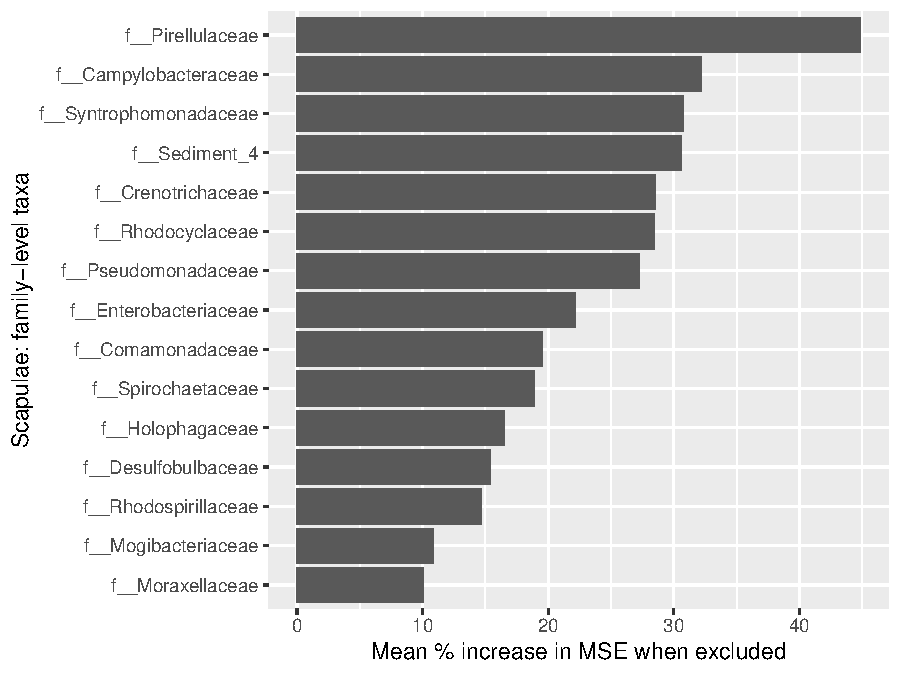
\includegraphics[width=3.25in]{use_families/w_scapulae/families_scapula_PercIncMSE_barchart}
    \end{figure}
  \end{center}
  \vspace{-0.1in}
  {\scriptsize
  \begin{itemize}
  \item I've shown 15 because they would fit, but 34 were used in the model.
  \item The first 7-8 taxa are noticeably more influential than those that
  follow.
  \end{itemize}
  }

\end{frame}



\begin{frame}{Scatterplots for influential taxa}

  \begin{center}
    \begin{figure}
      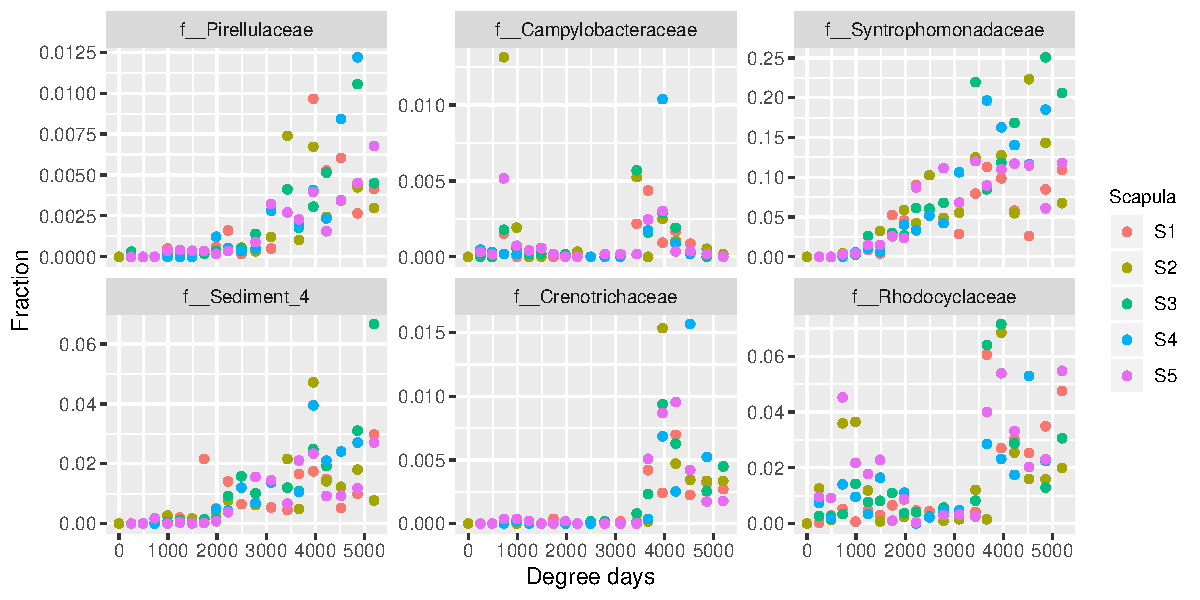
\includegraphics[width=4.75in]{use_families/w_scapulae/infl_scapula_family_scatter}
    \end{figure}
  \end{center}
  \vspace{-0.25in}
  {\scriptsize
  \begin{itemize}
  \item I've only shown top 6 because more than that is hard to fit.
  \item Note that the y-axes have differing scales.
  \item Fractions of Pirellulaceae, Campylobacteraceae, and Crenotrichacea
  are very low.
  \end{itemize}
  }

\end{frame}

\end{document}
